\documentclass{llncs}
\usepackage{makeidx}
\usepackage{amsmath}
\usepackage{amsfonts}
\usepackage{amssymb}
\usepackage[spanish]{babel}
\usepackage{graphicx}

%opening
\title{\large\huge Seminario\\ de \\Proyecto Modelos Aplicados\\ \small Tema:\\ \huge SexAppeal\\ \small En busca de una acto sexual ideal}
\author{ Integrantes: \\ Dayron Fernández Acosta C311\\ Javier Villar Alonso C311 \\ Julio José Horta C312\\ Daniel de la Cruz Prieto C311\\ }

\begin{document}

\maketitle
\newpage

\section{Introducción}
Desde el inicio de los tiempos siempre ha habido la necesidad de que los dos sexos (mujer y hombre) se relacionen con la finalidad de que en un futuro se casen y así la especie pueda perdurar, lo cual es un instinto. El apego a sus allegados se demostraba en la consideración que tenían con los muertos y la decoración del acto fúnebre, y el amor propio se notaba en sus vestimentas además de la preocupación por sus ornamentas. Por eso se puede afirmar que fue la base para la creación y el surgimiento del amor para lo cual necesitaban de la comunicación.
\newline
\newline
El amor es una construcción cultural y cada período histórico ha desarrollado una concepción diferente del amor. Y es muy importante mencionar que el tipo de amor que se presenta durante las relaciones amorosas es el amor romántico es cual se define como una manifestación de atracción física, entre dos personas, como la afinidad compartida por dos individuos, también podríamos decir que el amor es un sentimiento que comparten dos personas aleatorias que se encuentran y no pueden evitar atraerse entre sí. A pesar de que las relaciones amorosas de los adolescentes no siempre han tenido el mismo significado, siempre han estado presentes, y no solo durante la adolescencia, sino también en las otras etapas de la vida humana pero en los tiempos actuales, la adolescencia es la etapa donde mayormente se generan los noviazgos y es también donde se centra la problemática de la investigación que se realiza. 
\newline
\newline
En el momento que surge este interés amoroso, surge un fuerte deseo de actividad sexual entre la pareja inconscientemente, y a la vez una preocupación y a veces no logramos terminar como queremos una relación sexual.
\newline
\newline
En este trabajo abordaremos el problema de las relaciones sexuales y le daremos solución a diferentes modelos para que les sea más fácil realizar actos sexuales y puedan satisfacer siempre a su pareja


\section{Problema Analizado}
De un grupo que se reúne para realizar una actividad sexual nos interesa saber que secuencia para fomentar un resultado en específico, como lo es que el placer entre los individuos sea el máximo, o que el acto sexual dure el mayor tiempo posible, o hallar cual es el mejor resultado para que una cierta persona obtenga el mejor beneficio en ese acto sexual.
\newline
\newline
Para dar respuesta a este problema nos enfocamos en diversas variables:

\begin{tabular}{ccc}
	\textbf{posturas} & $\rightarrow$ & listas de las posturas disponibles para el grupo de personas\\
	\textbf{personas} & $\rightarrow$ & listas de las personas que realizarán el acto sexual\\
	
	\textbf{m} & $\rightarrow$ & Cantidad de personas\\
	\textbf{n} & $\rightarrow$ & Cantidad de posturas\\
	
	
	\textbf{personaXplacer (PGUT)} & $\rightarrow$ &  placer que le otorga a cada persona por cada posturas \\
	\textbf{personaXenergia (ECUT)} & $\rightarrow$ & energía que pierde cada persona por cada postura\\
	\textbf{enegiaInicial (EIP)} & $\rightarrow$ & Energía inicial de la persona\\
	\textbf{placerInicial (PIP)} & $\rightarrow$ & Placer inicial de la persona\\
	\textbf{placerRequerido (NPPOO)} & $\rightarrow$ & Placer Requerido de la persona para llegar al orgasmo\\
	\textbf{tiempoxpostura (T)} & $\rightarrow$ & tiempo dedicado para cada postura
\end{tabular}
\newline
\newline
\newline
Donde los modelos a estudiar serían los siguientes:
	
\section{Modelos}

\subsection{Maximizar la duración del acto sexual:}
En este caso nos interesa extender la duración de un acto sexual, lo que implica realizar el mayor tiempo de posturas que logre satisfacer a las personas que anden realizando el acto sexual y que cumplan con los requisitos suficientes para que todos estén satisfechos, para ello es necesario que realizaremos un modelo donde nos interesa maximizar la sumatoria de los tiempos dedicados a cada postura.
\newline
\newline
$Max$ $\sum_{i=1}^{m} T[i]$
\newline
\newline
Luego procedemos a trabajar las siguientes restricciones:

$1-)$ $\sum_{i=1}^{n} PGUT_{pi}t[i] \geq NPPOO_{p} - PIP_{p}$
\newline
\newline
Esta restricción expresa que el placer alcanzado por cada persona(p) entre 1 hasta m en las sumas de las posturas ejecutadas debe ser mayor o igual a lo necesario para llegar al orgasmo
\newline
\newline
$2-)$ $\sum_{i=1}^{n} ECUT_{pi}*t[i] \leq EIP_{pi}$
\newline
\newline
Esta restricción expresa que durante el acto sexual ninguna persona debe superar la energía que puede emplear en el acto sexual por cada persona(p) entre 1 hasta m


\subsection{Maximizar el placer del que menor placer alcance al finalizar el acto sexual:}
Para este modelo nos interesa encontrar a la persona que menor placer pueda alcanzar y proceder a maximizar su placer. Para ello maximizaremos una variable h que será el placer que alcance la persona h y mantendremos de variables los tiempos de cada postura.
\newline
\newline
$Max$ $h$
\newline
\newline
Luego le añadiremos las siguientes restricciones:
\newline
\newline
$1-)$ $\sum_{i=1}^{n} PGUT_{pi}*t_{i} \geq h - PIP_{p}$
\newline
\newline
En esta restricción expresa que la suma de los placeres alcanzados por las personas en el acto sexual debe de ser mayor o igual al placer alcanzado por el de menor placer menos la cantidad de placer necesaria para que alcance el orgasmo por cada persona(p) entre 1 hasta m
\newline
\newline
$2-)$ $\sum_{i=1}^{n} PGUT_{pi}t_{i} \geq NPPOO_{p} - PIP_{p}$
\newline
\newline
Esta restricción expresa que el placer alcanzado por cada persona(p) entre 1 hasta m en las sumas de las posturas ejecutadas debe ser mayor o igual a lo necesario para llegar al orgasmo
\newline
\newline
$3-)$ $\sum_{i=1}^{n} ECUT_{pi}*t_{i} \leq EIP_{pi}$
\newline
\newline
Esta restricción expresa que durante el acto sexual ninguna persona debe superar la energía que puede emplear en el acto sexual por cada persona(p) entre 1 hasta m


\subsection{Minimizar el cansancio del participante con mayor cansancio al finalizar el acto sexual:}
Este modelo es parecido al anterior, pero en este caso nos interesa minimizar el cansancio del que mayor cansancio alcanza al finalizar el acto sexual, la cual implica maximizar la energía de esta persona, para ello minimizaremos h y mantendremos como variables los tiempos de cada postura.
\newline
\newline
$Max$ $h$
\newline
\newline
Luego añadiremos las siguientes restricciones:
\newline
\newline
$1-)$ $\sum_{i=1}^{n} ECUT_{pi}*t_{i} \geq h - EIP_{pi}$
\newline
\newline
Donde expresamos que todas las personas desde 1 hasta m en el acto solo pueden gastar una energía mayor o igual a la diferencia entre la energía del que mayor cansancio acumula menos la energía inicial de la persona antes de comenzar el acto sexual
\newline
\newline
$2-)$ $\sum_{i=1}^{n} PGUT_{pi}t_{i} \geq NPPOO_{p} - PIP_{p}$
\newline
\newline
Esta restricción expresa que el placer alcanzado por cada persona(p) entre 1 hasta m en las sumas de las posturas ejecutadas debe ser mayor o igual a lo necesario para llegar al orgasmo
\newline
\newline
$3-)$ $\sum_{i=1}^{n} ECUT_{pi}*t_{i} \leq EIP_{pi}$
\newline
\newline
Esta restricción expresa que durante el acto sexual ninguna persona debe superar la energía que puede emplear en el acto sexual por cada persona(p) entre 1 hasta m

\subsection{Minimizar la energía inicial de todos los participantes de forma que al terminar todos hayan alcanzado el orgasmo y tengan la misma energía:}
En este modelo minimizaremos las energías iniciales de cada persona de forma que podamos igualar todas las energías de cada persona y llevaremos como variables el tiempo, las energías y un h que será el que menos energía alcance
\newline
\newline
$Min$ $\sum_{i=1}^{m} EIP_{i}$
\newline
\newline
Luego añadimos las siguientes restricciones:
\newline
\newline
$1-)$ $\sum_{i=1}^{n} ECUT_{pi}*t_{i} == EIP_{p} - h$
\newline
\newline
Donde buscamos un h tal que se igualen los EIP a la cantidad de energía gastada por las personas involucradas en el acto sexual. Siendo EIP variables no definidas. Además sin notan, al despejar el valor de EIP podemos verificar que el EIP de cada persona diferenciado con la energía gastada en el acto sexual por dicha persona, se volveran iguales a dicho h, lo que quiere decir que cada EIP - ECUT seran iguales el resultado para cada persona desde 1 hasta m
\newline
\newline
$2-)$ $\sum_{i = 1}^{n} ECUT_{pi}*t_{i} \leq EIP_{p}$
\newline
\newline
Esta restricción expresa que durante el acto sexual ninguna persona debe superar la energía que puede emplear en el acto sexual
\newline
\newline
$3-)$ $\sum_{i = 1}^{n} PGUT_{pi}*t_{p} \geq NPPOO_{p} - PIP_{p}$
\newline
\newline
Esta restricción expresa que el placer alcanzado por cada persona en las sumas de las posturas ejecutadas debe ser mayor o igual a lo necesario para llegar al orgasmo para cada persona entre 1 hasta m

\subsection{Maximizar el placer inicial de un participante específico, de forma tal que todos los participantes, excepto el específico, alcancen el orgasmo:}
Para este ejercicio trabajamos maximizando un h que indicará el placer de la persona definida por el usuario para maximizar su placer sin que llegue al orgasmo
\newline
\newline
$Max$ $H$
\newline
\newline
Con los tiempos como variables del problema y añadimos de restricciones las siguientes:
\newline
\newline
$1-)$ $\sum_{i = 1}^{n} ECUT_{pi}*t_{i} \leq EIP_{p}$
\newline
\newline
Donde buscamos que la energía gastada por las personas en el acto sexual para hacer las posturas sea menor o igual que la energía que tenía a disposición la persona para llevar a cabo toda la actividad por cada persona(p) de 1 hasta m
\newline
\newline
$2-)$ $\sum_{i = 1}^{n} PGUT_{pi}*t_{i} \geq NPPOO_{p} - PIP_{p}$
\newline
\newline
Esta restricción expresa que el placer alcanzado por cada persona(p) de 1 hasta m en las sumas de las posturas ejecutadas debe ser mayor o igual a lo necesario para llegar al orgasmo
\newline
\newline
$3-)$ $\sum_{i = 1} hPGUT_{i}*t_{i} < hNPPOO$
\newline
\newline
En esta restricción nos interesa que la persona definida(dicho h) en el modelo no alcance el orgasmo, por ello la cantidad de placer obtenida en el acto debe ser menor al placer requerido. La razon por la cual agregamos un h a una variable definida al inicio es para hacer referencia a la persona definida
\newline
\newline
$4-)$ $hNPPOO > h$
\newline
\newline
En esta restricción buscamos maximizar el placer de h pero imponiendo que no pueda superar el placer requerido para llegar al orgasmo
\newline
\newline
$5-)$ $\sum_{i = 1}^{n} PGUT_{pi}*t_{i} \geq NPPOO_{p} - PIP_{p}$
\newline
\newline
Esta restricción expresa que el placer alcanzado por cada persona en las sumas de las posturas ejecutadas debe ser mayor o igual a lo necesario para llegar al orgasmo

\newpage

\section{Programación los modelos}	
En este trabajo usamos la biblioteca pulp, un repo muy usado en la optimización de modelos que nos facilitará hallar los resultados de nuestro problema. Esta implica en la construcción del modelo mediante clasificaciones y agregándolo a una variable que nos permitirá procesar el problema
\newline
\newline
PuLP permite indicar el tipo de problema que hay que optimizar mediante palabras reservadas de la propia librería, maximización (LpMaximize) o minimización (LpMinimize), que deberán usarse cuando comenzamos a definirlo. Además, incluye soporte base para todos y cada uno de los elementos básicos de un problema de optimización:
\newline
\newline
- Variables (LpVariable): la cual usaremos para declarar las variables de nuestro modelo
\newline
- Función objetivo
\newline
- Restricciones o constraints
\newpage
\subsection{Código de los modelos:}

\begin{figure}
	\centering
	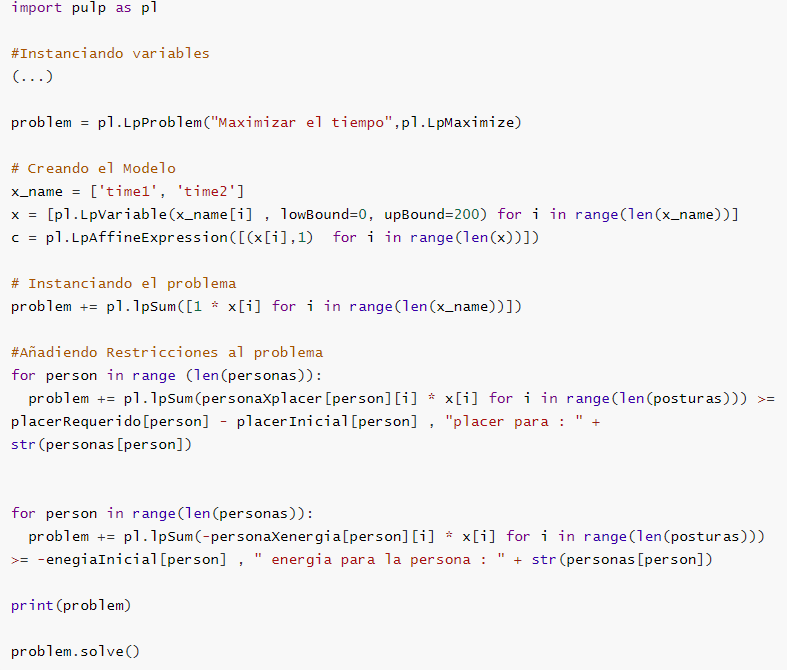
\includegraphics[width=0.7\linewidth]{Imagenes/modelo1-Guia}
	\label{fig:modelo1-guia}
\end{figure}

Dicho código representa el primer modelo de nuestro problema y su forma de trabajar es sencilla. Primero instanciamos las variables fijas que queremos tener para luego plantear el tipo de modelo que queremos efectuar, ya sea de minimización o maximización usando la sintaxis LpMinimize o LpMaximize a la hora de instanciar el LpProblem que es donde guardaremos todo nuestro modelo
\newline
\newline
Luego para este caso procedemos a instanciar el problema que debemos resolver la cual en este caso buscamos maximizar la suma de los tiempos de un acto sexual
\newline
\newline
Luego seguiría instanciar nuevas variables en el caso que no solo se quieran las variables del modelo que queremos proceder a calcular usando LpVariable pero para este caso no es necesario y solo pasaremos al siguiente paso
\newline
\newline
En el siguiente paso vamos agregando poco a poco al problema las restricciones que definen al modelo del problema
\newline
\newline
Ya luego de haber seguido estos pasos podemos mandar a imprimir sus valores y enviar el resultado obtenido
\newpage

\begin{figure}
	\centering
	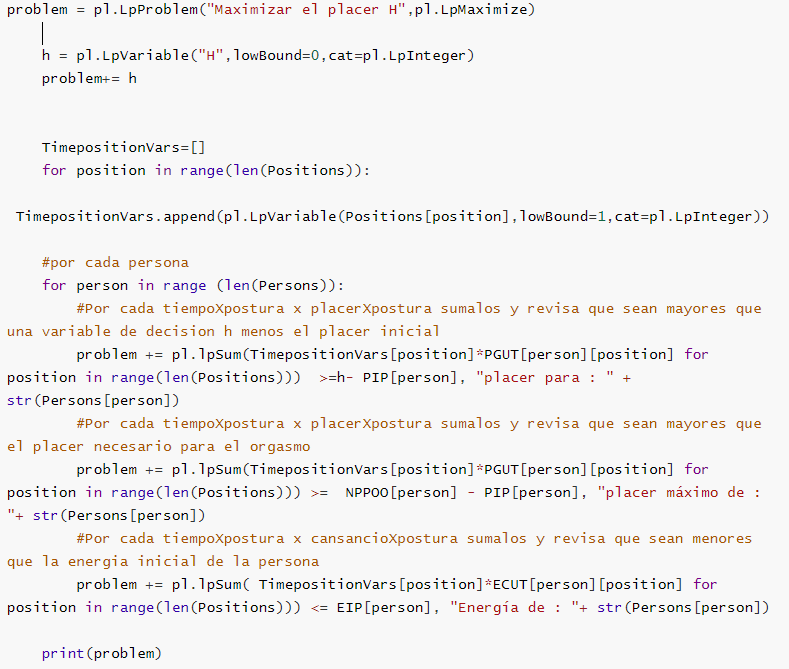
\includegraphics[width=0.7\linewidth]{Imagenes/modelo2-Guia}
	\label{fig:modelo2-guia}
\end{figure}

En este modelo que radica en lo que hablamos del modelo 2 podemos ver que la forma de proceder que explicamos en la anterior imágenes es similar, lo unico que ya aqu'i usaremos las LpVariables que planteamos anteriormente, la cual nos sirve para plantear variables fuera del modelo principal
\newline
\newline
Para los próximos modelos los programaríamos de manera muy similar

\newpage

\section{Modelos Duales}
Ya como conocemos los modelos originales entonces para hallar los modelos duales solo es necesario modificar modelos y hacer transpuesta para poder hallar los modelos duales, ya que el procedimiento de calcularlos es mediante hallar pares de números que al multiplicar las restricciones se conviertan en la menor cota que podamos comparar con nuestra función modelo
\newline
\newline
Dicho esto podemos proceder a ver nuestros modelos duales:

\subsection{Variables}

n : cantidad de posturas
\newline
m : cantidad de personas

\subsection{Modelo N1}
$Min$ $\sum_{i=1}^{m} \lambda_{ix}*EIP_{i} + \sum_{j = 0}^{m} \lambda_{iy}(NPPOO_{i} - PIP_{i})$
\newline
\newline
Restricciones:
\newline
$(1)$  $\sum_{i = 1}^{m} \lambda_{ix}ECUT_{ix1} + \sum_{j = 0}^{m} \lambda_{iy}PUGT_{ix1} \leq 1$
\newline
$(j)$ $\sum_{i = 1}^{m} \lambda_{ix}ECUT_{ixj} + \sum_{j = 0}^{m} \lambda_{iy}PUGT_{ixj} \leq 1 $
\newline
Para todo j que pertenece a posturas
\newline
\newline
$\lambda_{ix} \geq 0$ , $\lambda_{jy} \leq 0$

\subsection{Modelo N2}
$Min$ $\sum_{i = 1}^{m} \lambda_{ix}EIP_{i} + \sum_{j = 0}^{m} \lambda_{jy}(NPPOO_{j}-PIP_{j}) + \sum_{h = 0}^{m} \lambda_{hz}(-PIP_{h})$
\newline
\newline
Restricciones:
\newline
$(1)$  $\sum_{i = 1}^{m} \lambda_{ix}ECUT_{i1} + \sum_{i = 0}^{m} \lambda_{iy}PUGT_{i1} + \sum_{h = 0}^{m}\lambda_{hz}PUGT_{h1}\leq 0$
\newline
$(j)$ $\sum_{i = 1}^{m} \lambda_{ix}ECUT_{ij} + \sum_{i = 0}^{m} \lambda_{iy}PUGT_{ij} + \sum_{h = 0}^{m}\lambda_{hz}PUGT_{hj} \leq 0 $
\newline
Para todo j que pertenece a posturas
\newline
\newline
$(m+1)$ $\sum_{i = 1}^{m} -\lambda_{ih}  \leq 1$
\newline
\newline
$\lambda_{ix} \geq 0$ , $\lambda_{jy} \leq 0, \lambda_{hz} \leq 0$

\subsection{Modelo N3}
$Min$ $\sum_{i = 1}^{m} \lambda_{ix}EIP_{i} + \sum_{j = 0}^{m} \lambda_{jy}(NPPOO_{j}-PIP_{j}) + \sum_{h = 0}^{m} \lambda_{hz}(-PIP_{h})$
\newline
\newline
Restricciones:
\newline
$(1)$  $\sum_{i = 1}^{m} \lambda_{ix}ECUT_{i1} + \sum_{j = 0}^{m} \lambda_{iy}PUGT_{i1} + \sum_{h = 0}^{m}\lambda_{hz}PUGT_{h1}\leq 0$
\newline
$(j)$ $\sum_{i = 1}^{m} \lambda_{ix}ECUT_{ij} + \sum_{i = 0}^{m} \lambda_{iy}PUGT_{ij} + \sum_{h = 0}^{m}\lambda_{hz}PUGT_{hj} \leq 0 $
\newline
Para todo j que pertenece a posturas
\newline
\newline
$(m+1)$ $\sum_{i = 1}^{m} \lambda_{jy}  \leq 1$
\newline
\newline
$\lambda_{ix} \geq 0$ , $\lambda_{jy} \leq 0, \lambda_{hz} \leq 0$

\subsection{Modelo N4}
$Max$ $\sum_{j = 1}^{m} \lambda_{jy}(NPPOO_{j} - PIP_{j})$
\newline
\newline
Restricciones:
\newline
$(1)$  $\sum_{i = 1}^{m} \lambda_{ix}ECUT_{i1} + \sum_{i = 0}^{m} \lambda_{iy}PUGT_{i1} + \sum_{h = 0}^{m}\lambda_{hz} \leq 0$
\newline
$(...)$
\newline
$(m+1)$  $ - \sum_{i = 1}^{m} \lambda_{ix}EIP_{i1} - \sum_{h = 0}^{m}\lambda_{hz}EIP_{h} \leq 1$
\newline
$(m+2)$ $\sum_{i = 0}^{m} \lambda_{ih} H  \leq 0$

\subsection{Modelo N5}
$Min$ $NPPOO_{i}\lambda$
\newline
\newline
$\lambda \leq 1$
\newline
$\lambda \geq 0$

\subsection{Interpretación general de los Duales}
En los primeros 3 problemas primales tendremos n variables, una por cada posición del acto. Mientras que con respecto a sus restricciones, por cada persona m se encuentran 2 restricciones, una que trata el placer y otra la energía. Por tanto al hallar el dual, terminamos con un problema de optimización con el que tendremos 2m variables objetivo y n restricciones.
\newline
\newline
El problema Dual del modelo uno se puede interpretar como la minimización de la suma entre las Energías Iniciales de cada participante y su placer necesario para alcanzar el orgasmo, cumpliendo que para cada una de las posturas la sumatoria de las energías y placeres utilizado en esa postura por todos los participantes sea la menor posible.
\newline
\newline
Para la interpretación del modelo 2, debemos tener en cuenta que nos encontramos en el primal con 3 restricciones por persona, lo cual hará que nuestro Dual esté compuesto por 3m variables de decisión. Sin embargo, las restricciones están dadas, no solo por las n variables del primal, sino además por una restricción más dada por la variable H. La función objetivo del dual y sus restricciones mantienen una interpretación parecida al Dual anterior, con la diferencia de que el placer también dependerá de una nueva variable lambda dada por H, y una nueva restricción de que la sumatoria de estos lambda debe ser menor o igual que 1. En el Dual 3, todo es mantenido de igual manera, con la diferencia de que las lambda dadas por H en este caso afectan al comportamiento de la Energía en lugar del Placer.
\newline
\newline
El Dual 4 presenta la idea de maximizar la sumatoria de los niveles de placer que debe ser generado por postura para cada participante mientra se mantiene que sus energías iniciales y finales sean lo mas cercana posible.
\newline
\newline
El modelo 5 y su dual son distintos a todos los anteriores, en el sentido que no tendremos una restricción por cada una de las posturas involucradas en el acto. Pues aunque las restricciones deben seguir cumpliéndose, todas ellas excepto las de una persona, no dependen de ninguna variable objetivo. Todas se vuelven restricciones compuestas por constantes. La única restricción mantenida, es que la sumatoria del placer generado en cada postura del participante i , mas su placer inicial H (variable de decisión) no sea suficiente para alcanzar el orgasmo. El dual terminará dado por un lambda positivo que minimice el valor de la diferencia entre el placer necesario para alcanzar el orgasmo y la sumatoria del placer generado por postura. 



\section{Aplicación Presentada}
La aplicación consiste en una página web hecha con streamlit donde nos permitirá proceder a realizar estos modelos agregando datos a nuestra conveniencia y obtener un resultado de acuerdo a la consulta mandada por el usuario 

\subsection{Guía técnica de la aplicación}
Para uso de la aplicación es necesario tener instalados los siguientes requerimientos:
\newline
\newline
beautifulsoup4 == 4.10.0
\newline
numpy == 1.22.1
\newline
pandas == 1.3.5
\newline
PuLP == 2.6.0
\newline
scipy == 1.7.3
\newline
streamlit == 1.4.0
\newline
\newline
streamlit-option-menu
\newline
\newline
hydrali$\_$components

Luego de todo esto iniciaremos por consola cmd desde la carpeta de la aplicación con el comando streamlit run sexapp.py
\newline
\newline
Una vez hecho deberá aparecer la siguiente pagina web:

\begin{figure}
	\centering
	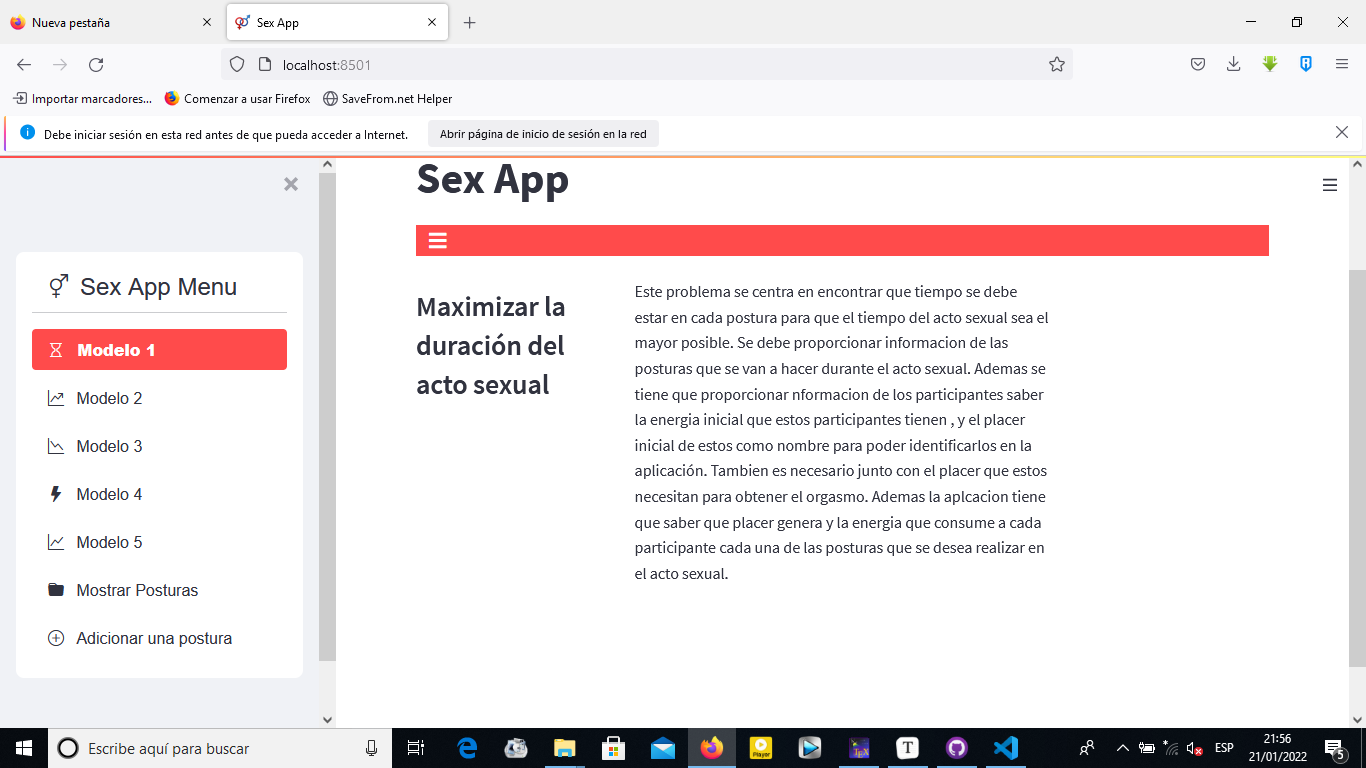
\includegraphics[width=0.7\linewidth]{Imagenes/aplicacion/web1}
	\label{fig:web1}
\end{figure}

Esta página web es nuestra aplicación que consiste en un formulario en la que elegirás los datos a conveniencia y rellenarás información necesaria para poder operar la aplicación.
\newline
\newline
Para eso primero que nada podemos ver que en la barra izquierda podemos seleccionar un grupo de opciones donde 5 de ellos son los modelos a disposición para la aplicación, una opción para ver las posturas a disposición y otra opción para crear nuevas posturas que queramos usar en nuestra aplicación:

\begin{figure}
	\centering
	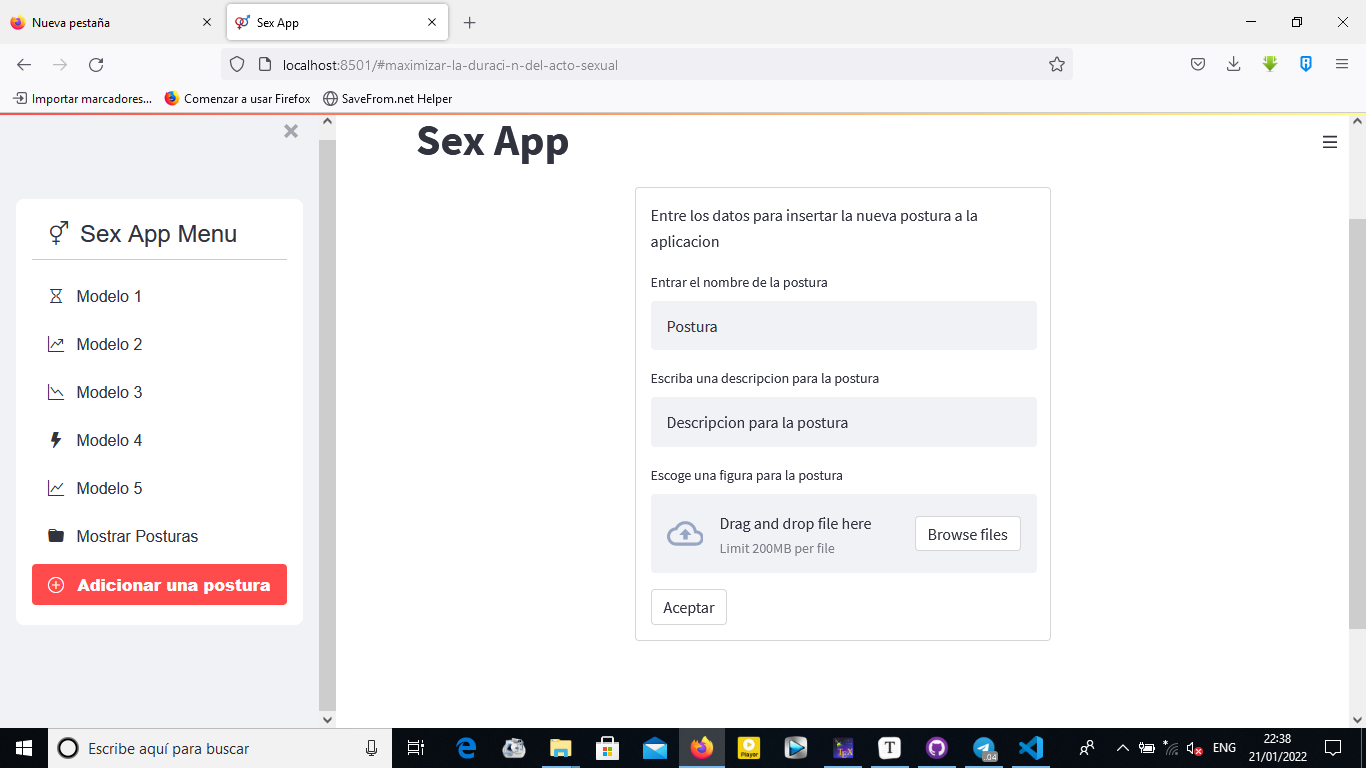
\includegraphics[width=0.7\linewidth]{Imagenes/aplicacion/web2}
	\label{fig:web2}
\end{figure}
\begin{figure}
	\centering
	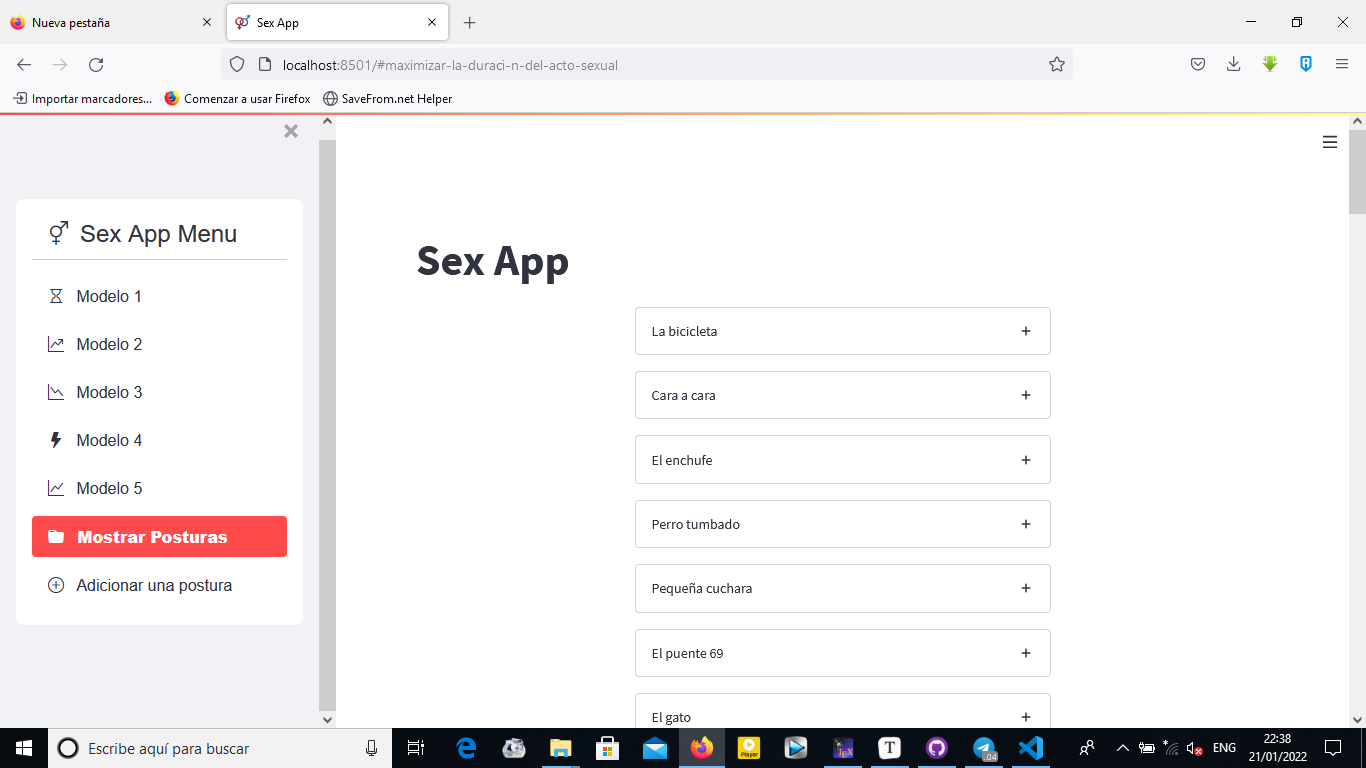
\includegraphics[width=0.7\linewidth]{Imagenes/aplicacion/web3}
	\label{fig:web3}
\end{figure}
\begin{figure}
	\centering
	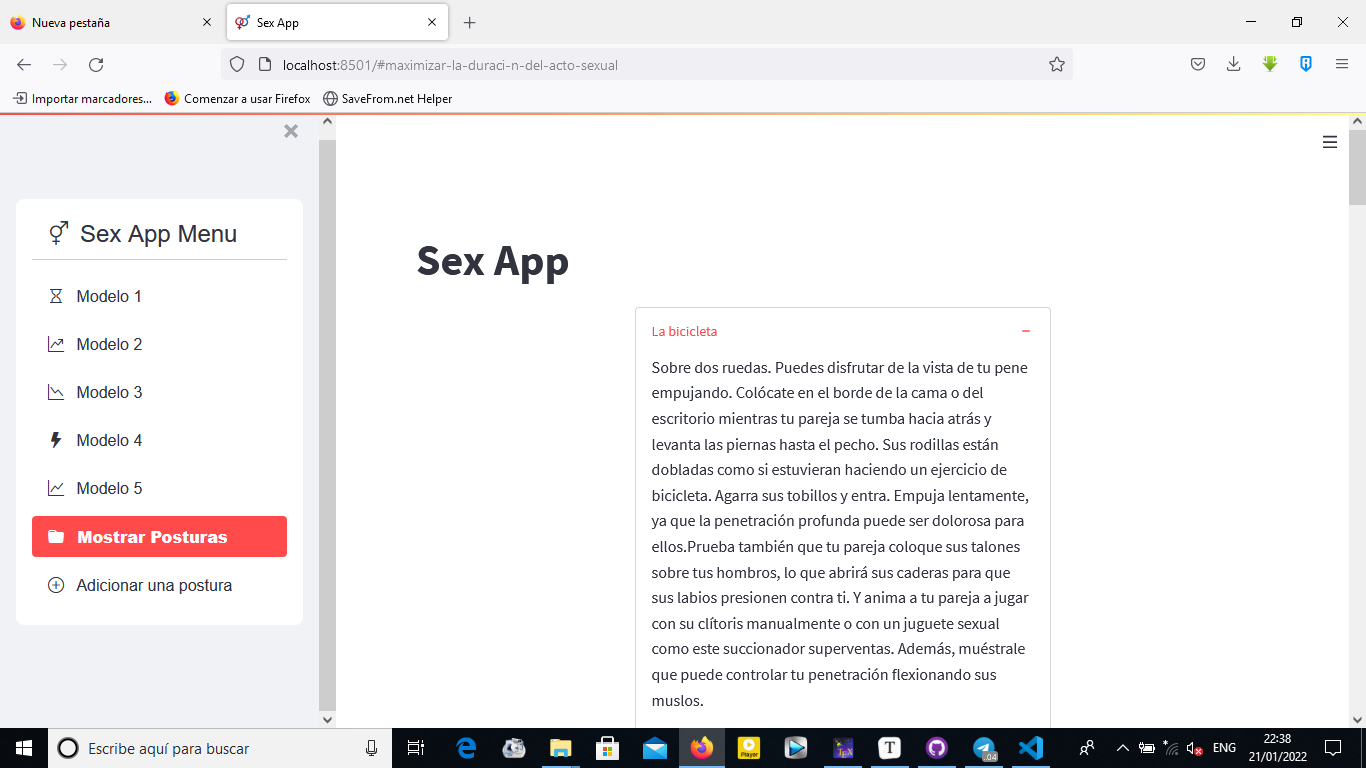
\includegraphics[width=0.7\linewidth]{Imagenes/aplicacion/web4}
	\label{fig:web4}
\end{figure}

Volvamos a modelos1:
\begin{figure}
	\centering
	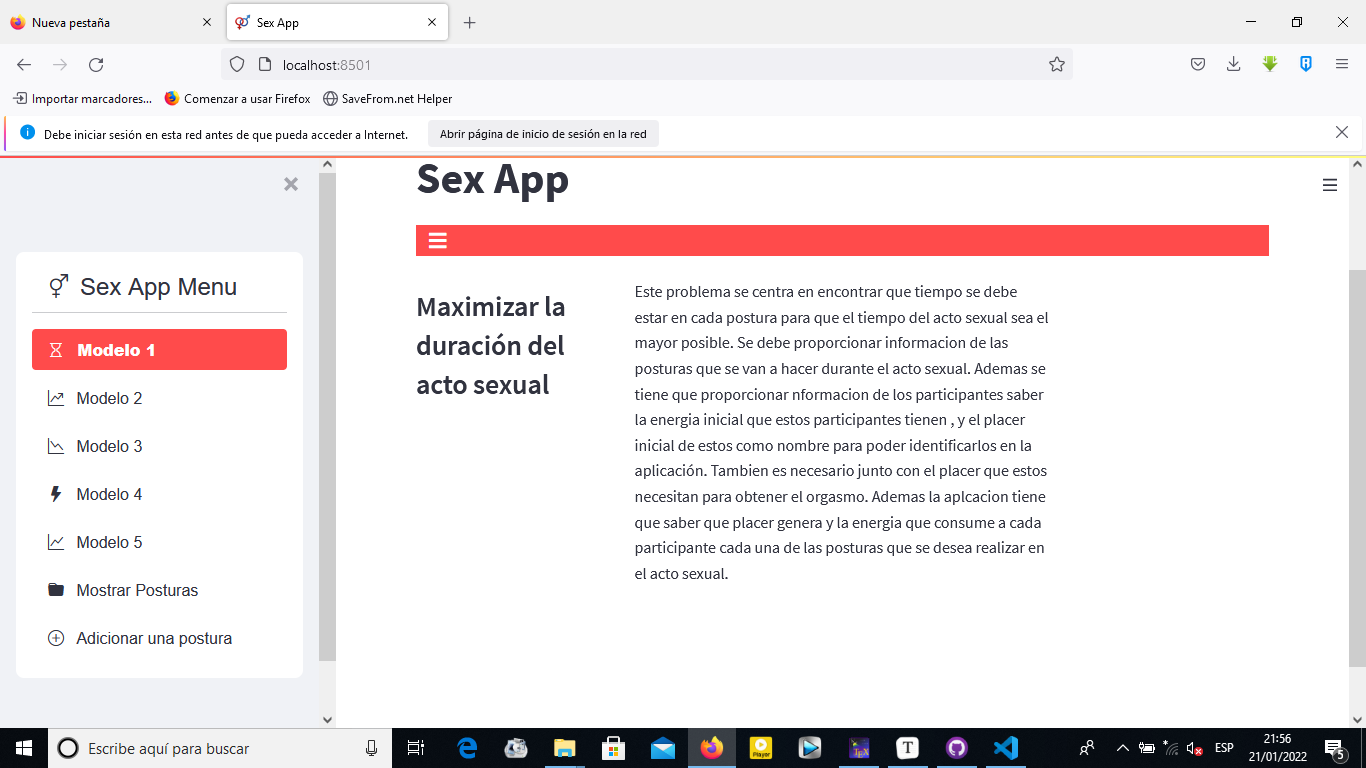
\includegraphics[width=0.7\linewidth]{Imagenes/aplicacion/web1}
	\label{fig:web1.1}
\end{figure}

Si nos percatamos también nos sale una barra en la parte superior que cuando la expandimos nos salen un grupo de opciones:

\begin{figure}
	\centering
	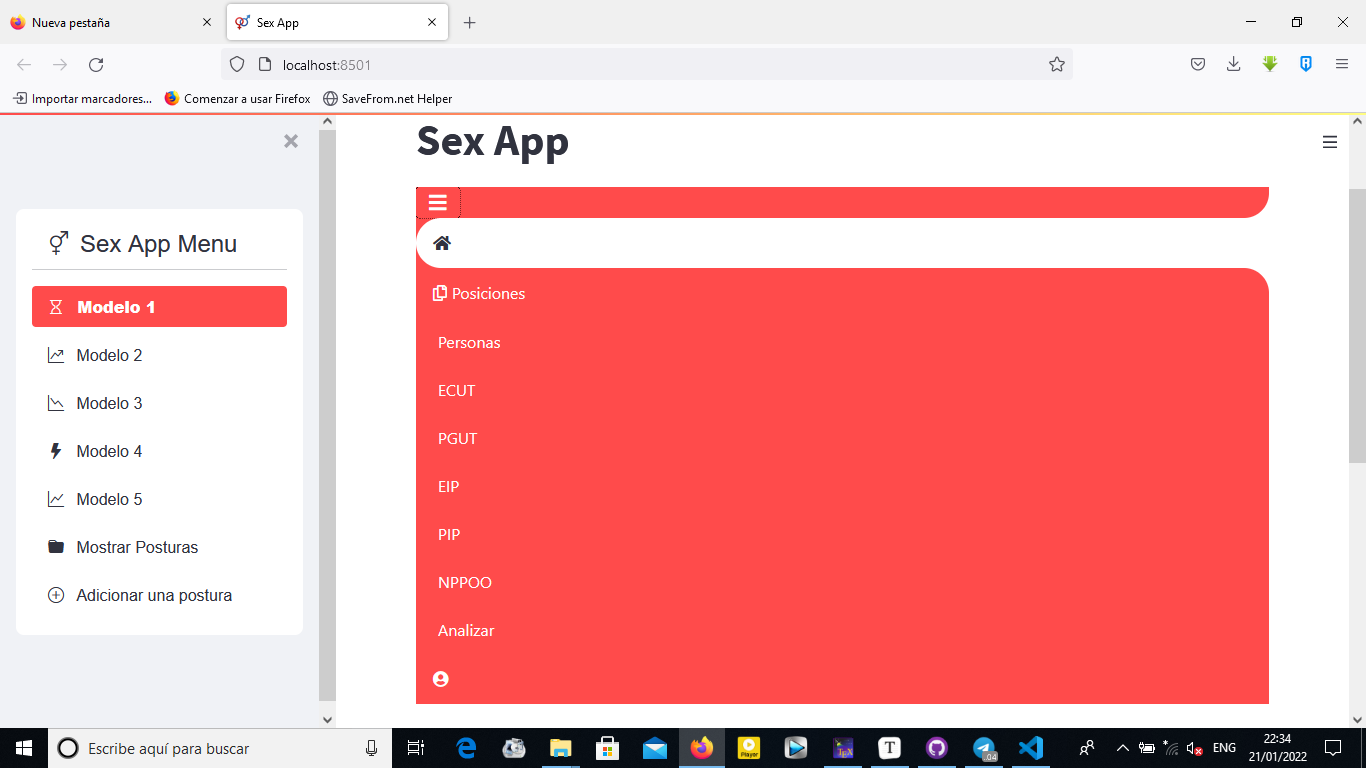
\includegraphics[width=0.7\linewidth]{Imagenes/aplicacion/web5}
	\label{fig:web5}
\end{figure}

Si vamos a personas podemos agregar participantes para el acto sexual:

\begin{figure}
	\centering
	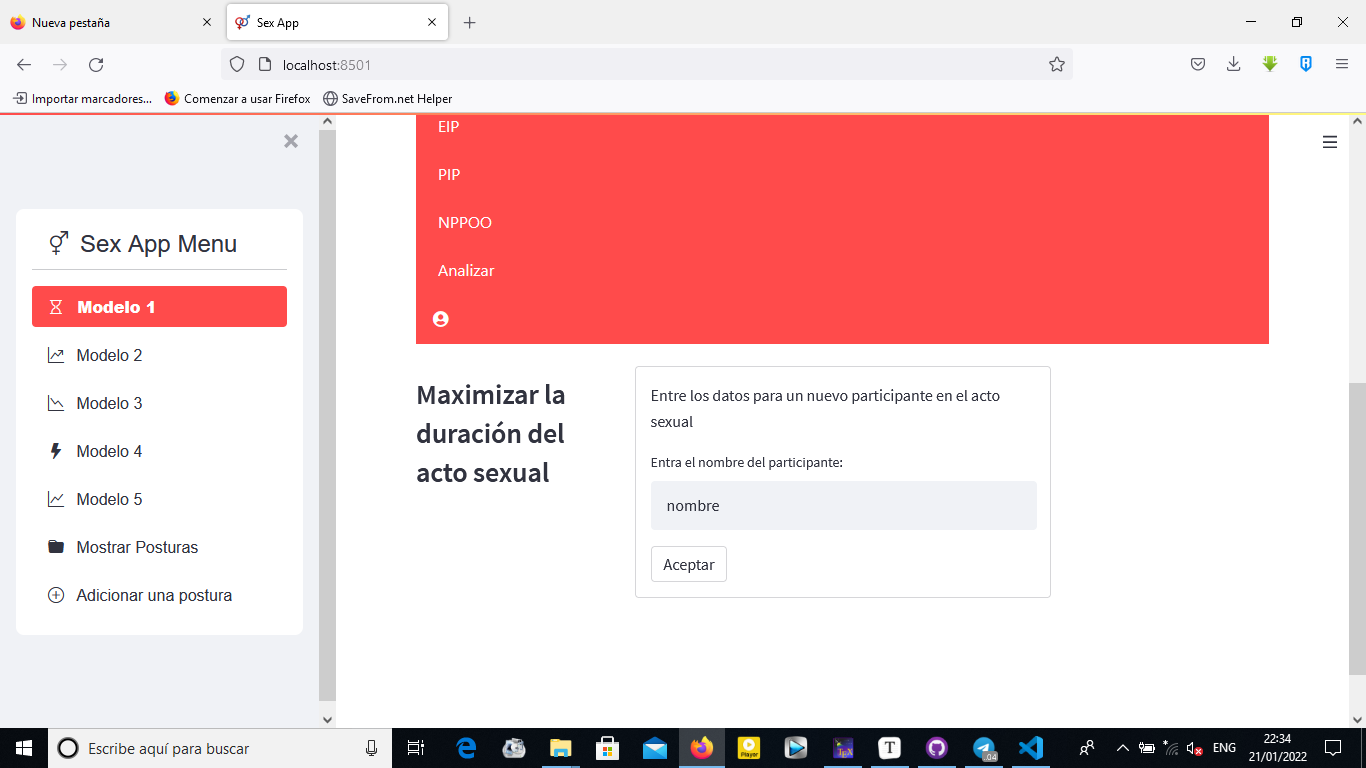
\includegraphics[width=0.7\linewidth]{Imagenes/aplicacion/web6}
	\label{fig:web6}
\end{figure}
\begin{figure}
	\centering
	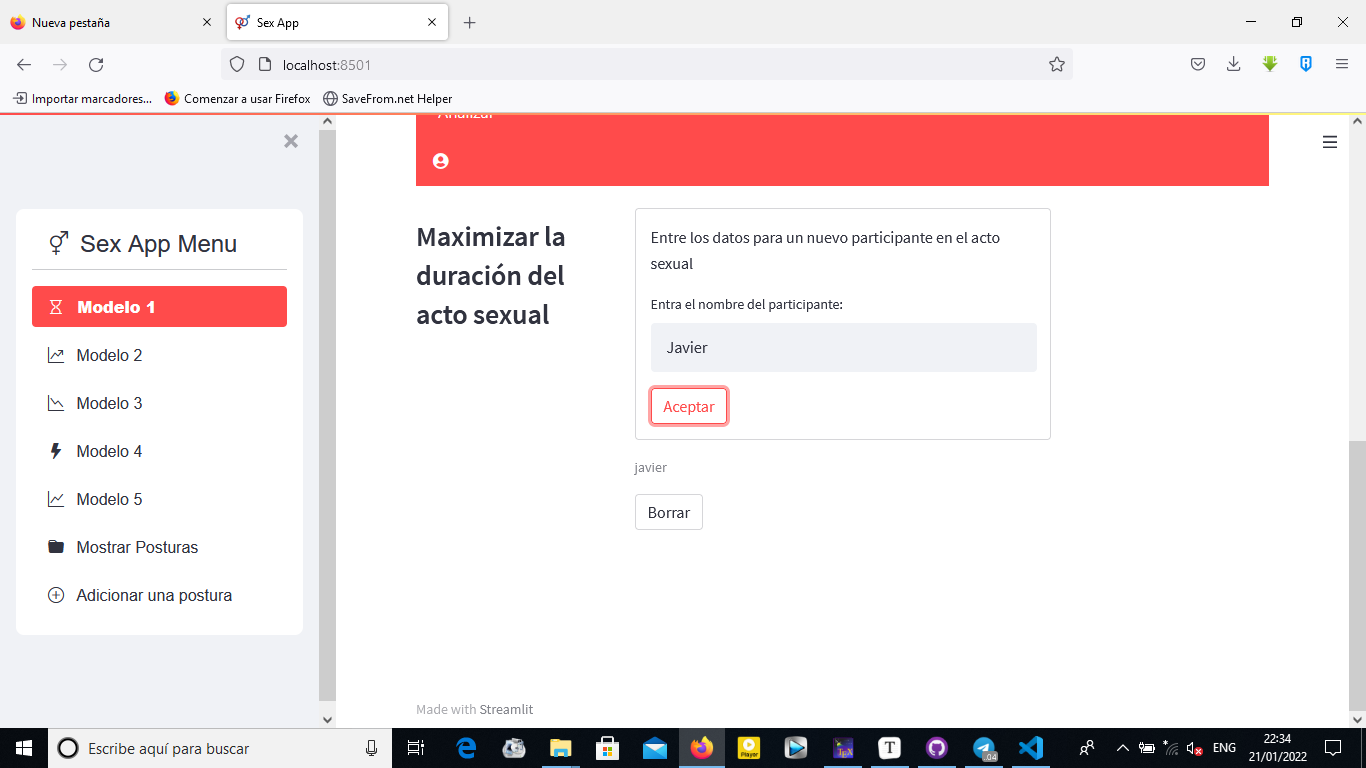
\includegraphics[width=0.7\linewidth]{Imagenes/aplicacion/web7}
	\label{fig:web7}
\end{figure}

Si vamos a posturas podemos seleccionar las posturas que están disponibles para el acto sexual de las que hemos guardado en la aplicación:

\begin{figure}
	\centering
	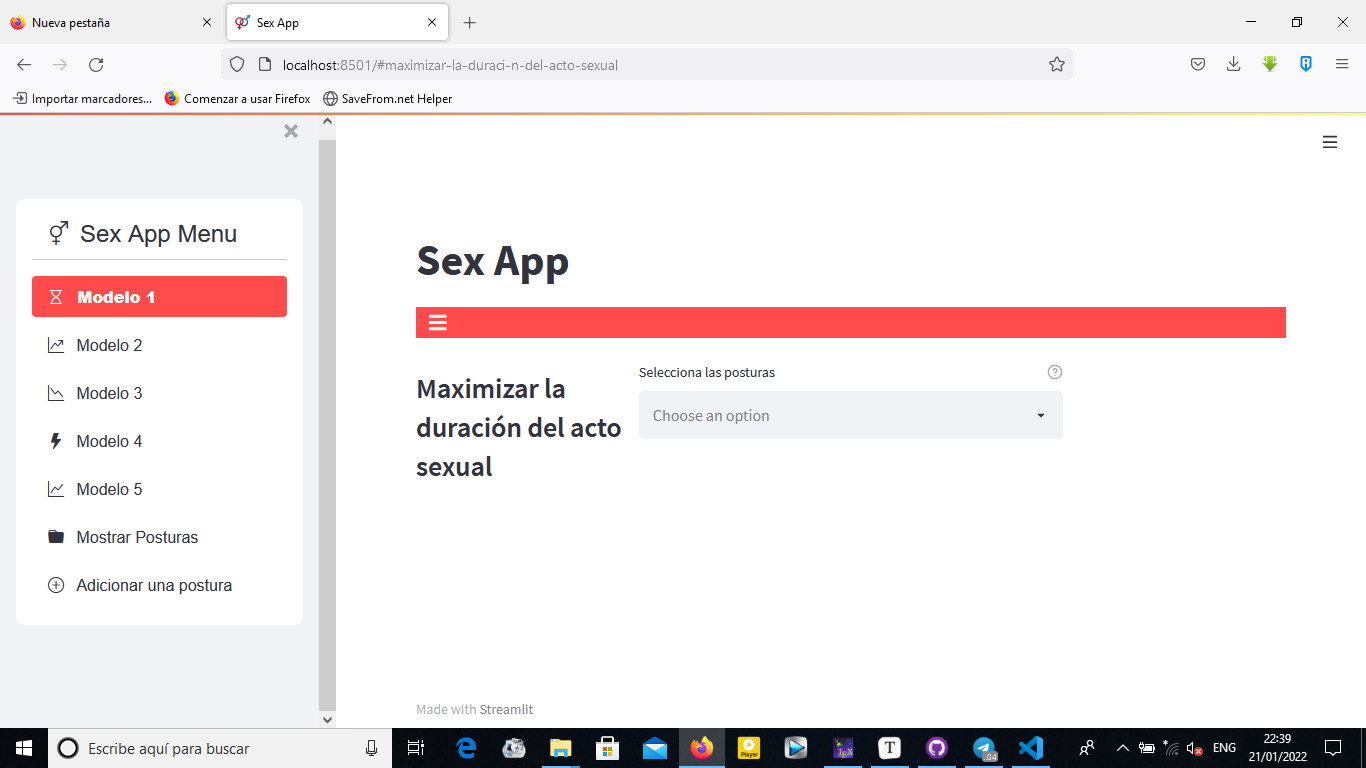
\includegraphics[width=0.7\linewidth]{Imagenes/aplicacion/web8}
	\label{fig:web8}
\end{figure}
\begin{figure}
	\centering
	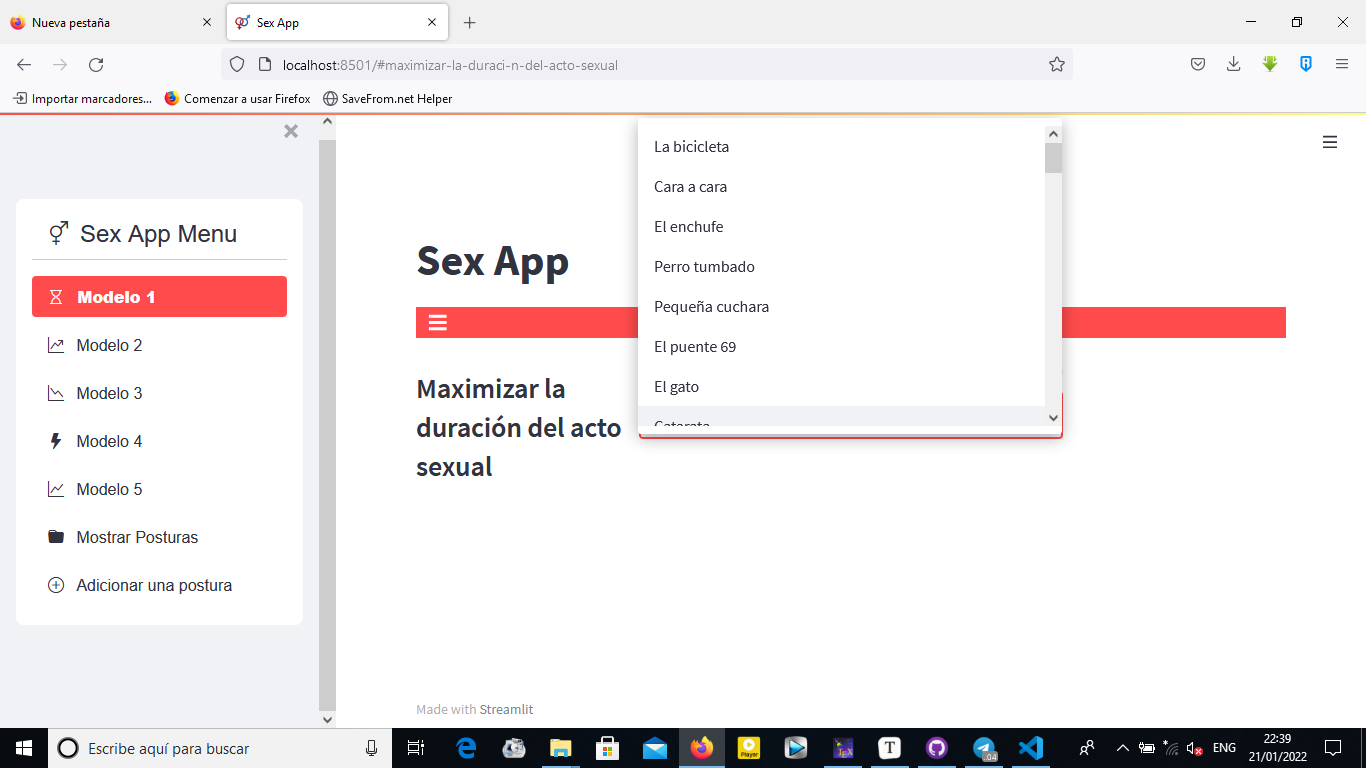
\includegraphics[width=0.7\linewidth]{Imagenes/aplicacion/web9}
	\label{fig:web9}
\end{figure}
\begin{figure}
	\centering
	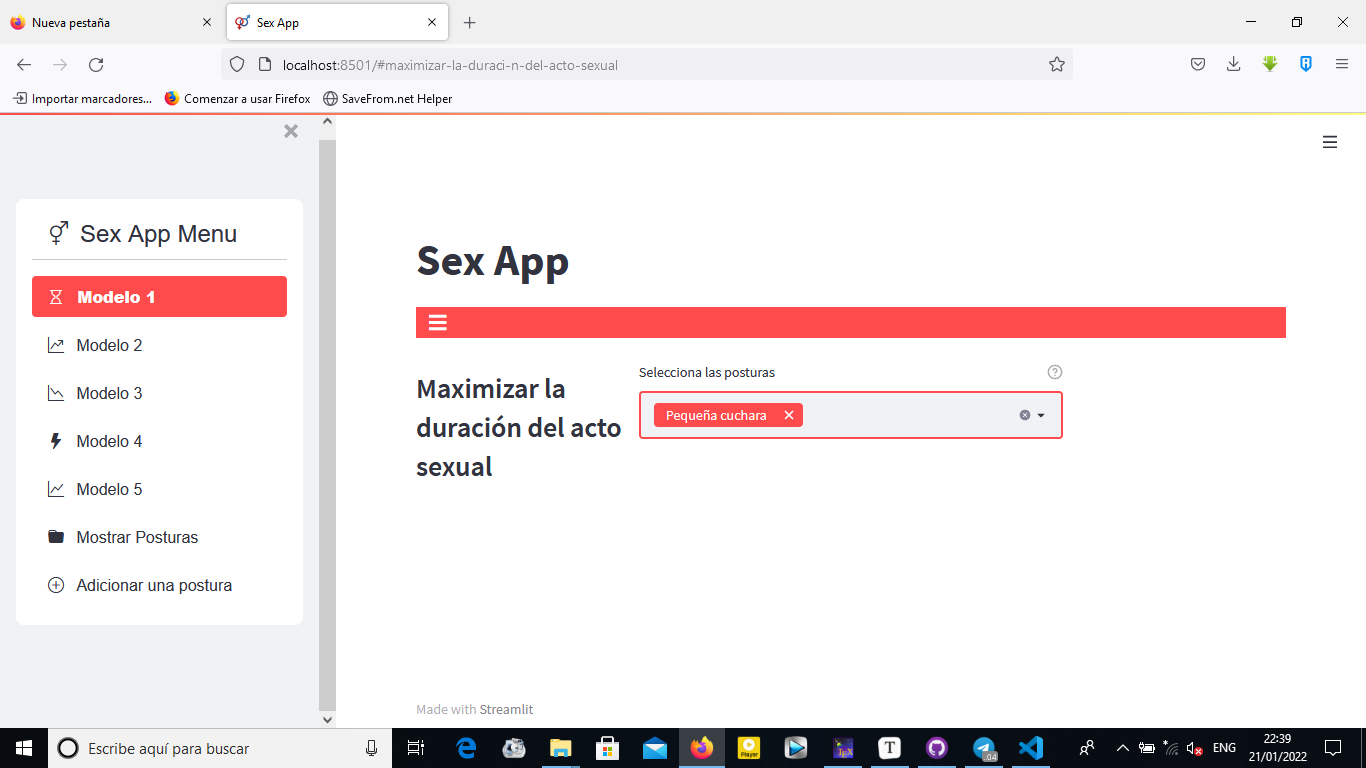
\includegraphics[width=0.7\linewidth]{Imagenes/aplicacion/web10}
	\label{fig:web10}
\end{figure}

Si queremos eliminar de las elegidas alguna solo debemos tocar la X que sale en el nombre del que escogimos o agregamos (también es disponible dicha opción para personas)
\newline
\newline
Si vamos ECUT, PGUT podemos ajustar sus datos de acuerdo a las posturas que añadimos al acto sexual disponibles para cada persona creada:

\begin{figure}
	\centering
	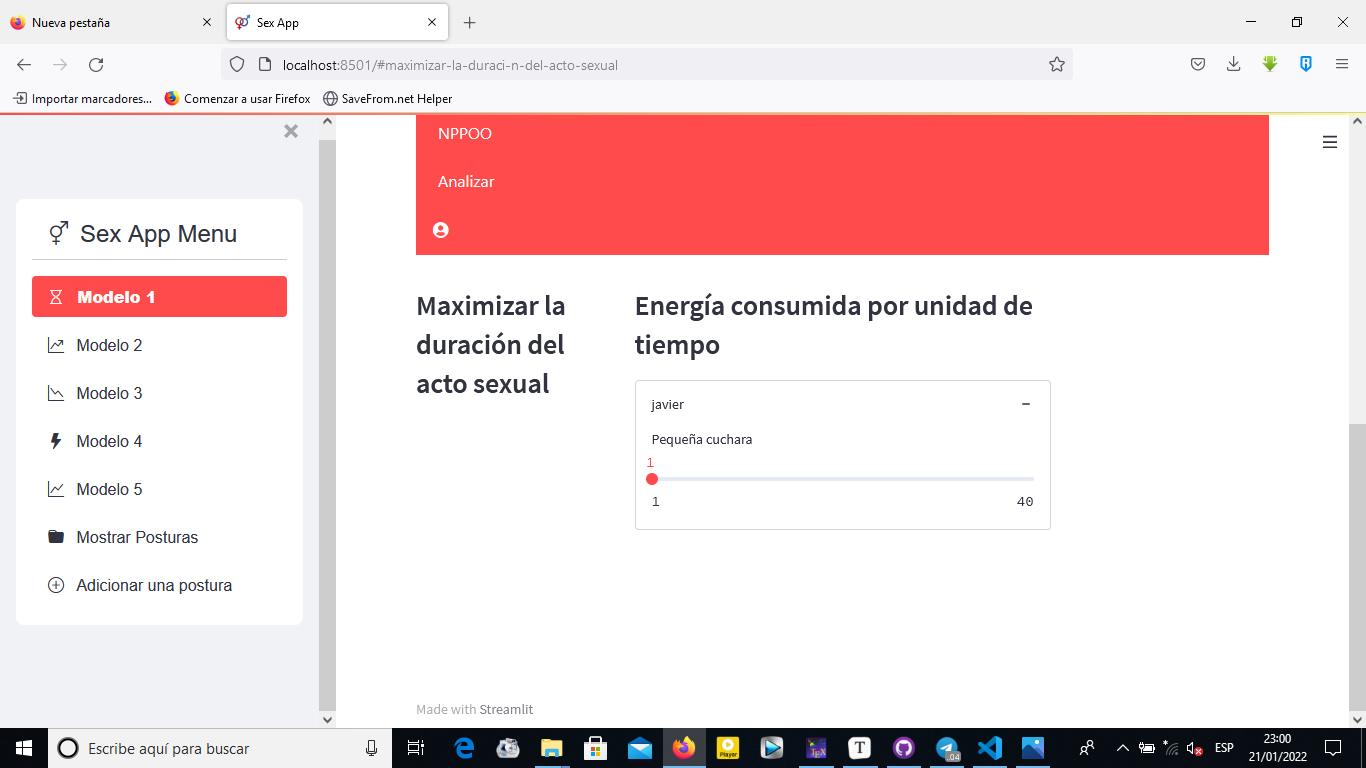
\includegraphics[width=0.7\linewidth]{Imagenes/aplicacion/web11}
	\label{fig:web11}
\end{figure}

Si vamos a las opcione EIP, PIP y NPPOO podemos ajustar datos también de acuerdo a las personas que añadimos

\begin{figure}
	\centering
	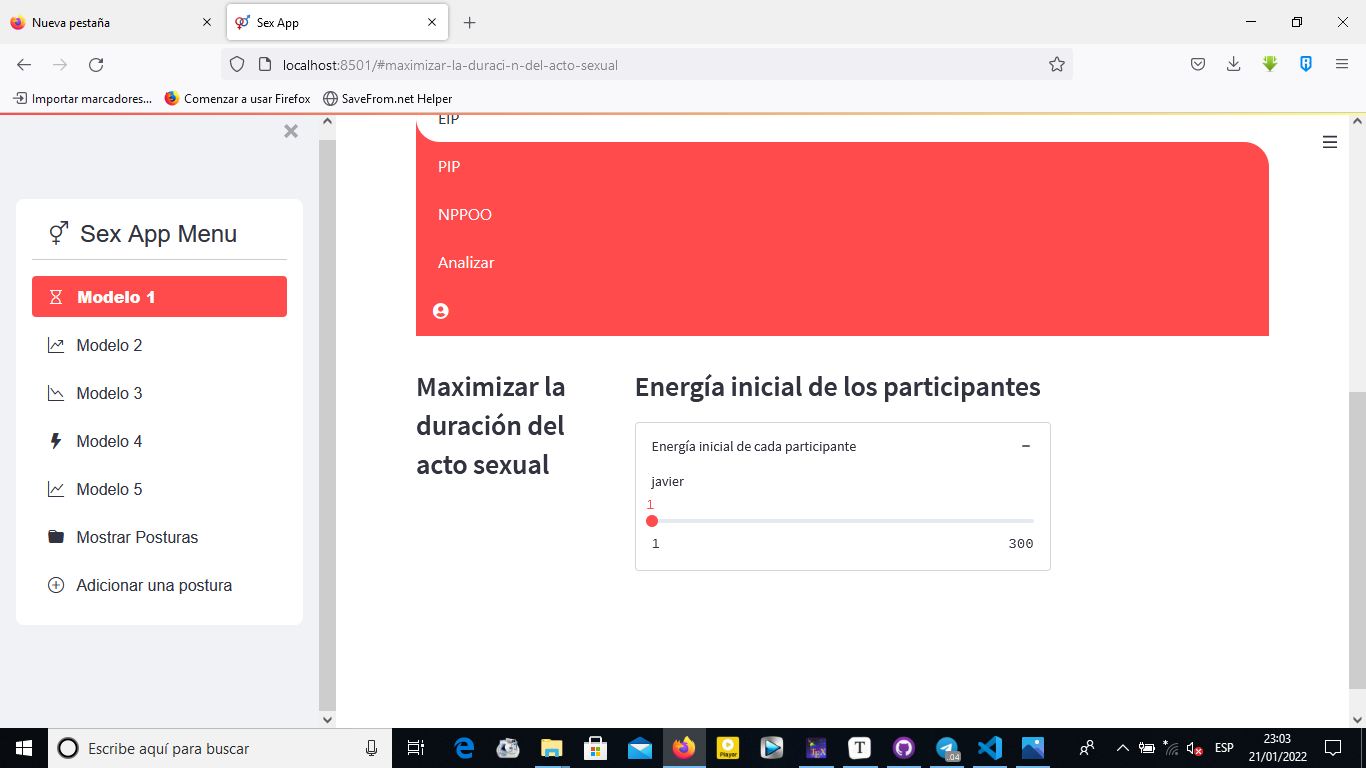
\includegraphics[width=0.7\linewidth]{Imagenes/aplicacion/web12}
	\label{fig:web12}
\end{figure}
\begin{figure}
	\centering
	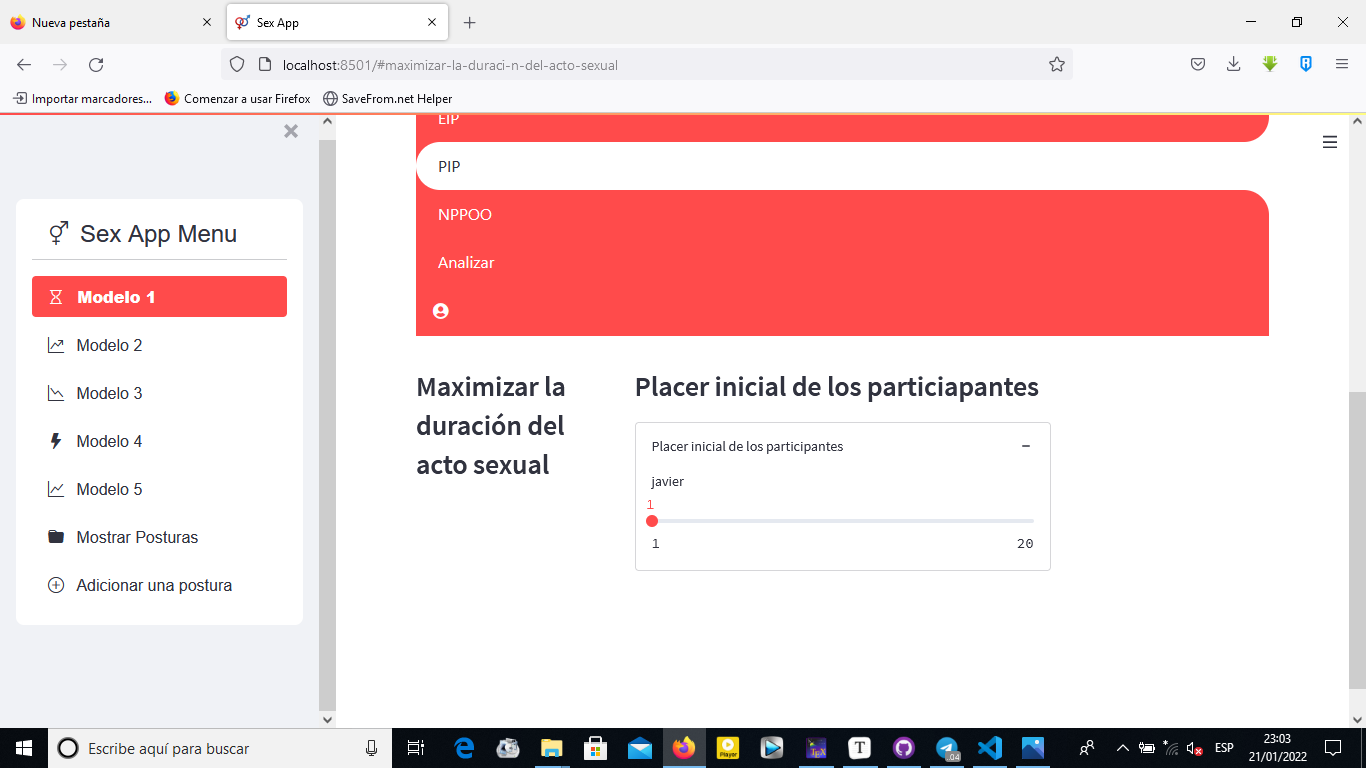
\includegraphics[width=0.7\linewidth]{Imagenes/aplicacion/web13}
	\label{fig:web13}
\end{figure}
\begin{figure}
	\centering
	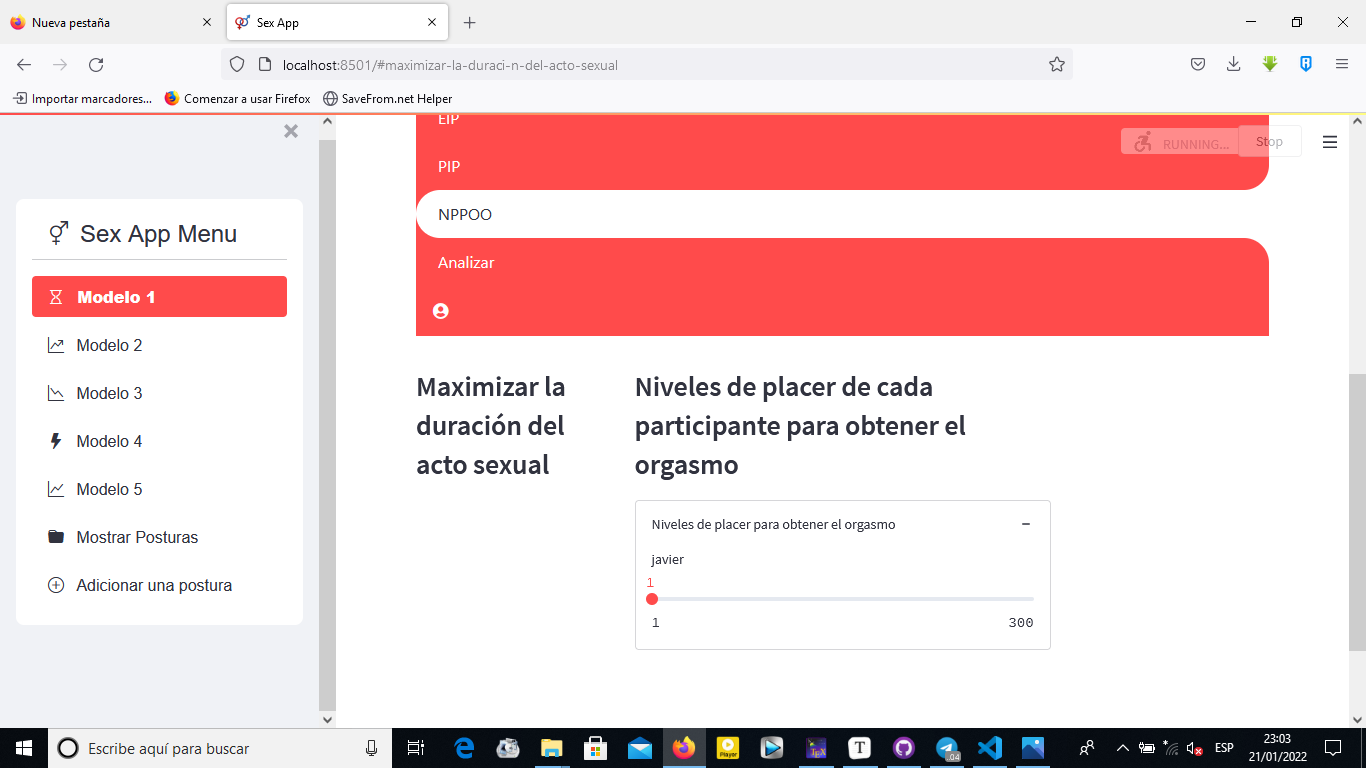
\includegraphics[width=0.7\linewidth]{Imagenes/aplicacion/web14}
	\label{fig:web14}
\end{figure}

Además que cada una de esas 5 opciones planteadas anteriormente cuentan con una breve descripción del tipo de dato que describen en el modelo
\newline
\newline
Una vez ingresado los datos queridos aparece una opción llamada "analyce" que es para ejecutar nuestro problema, donde si encuentra un resultado válido a nuestros datos ingresados entonces imprimirá una serie de gráficos de comportamiento de nuestros datos:

\begin{figure}
	\centering
	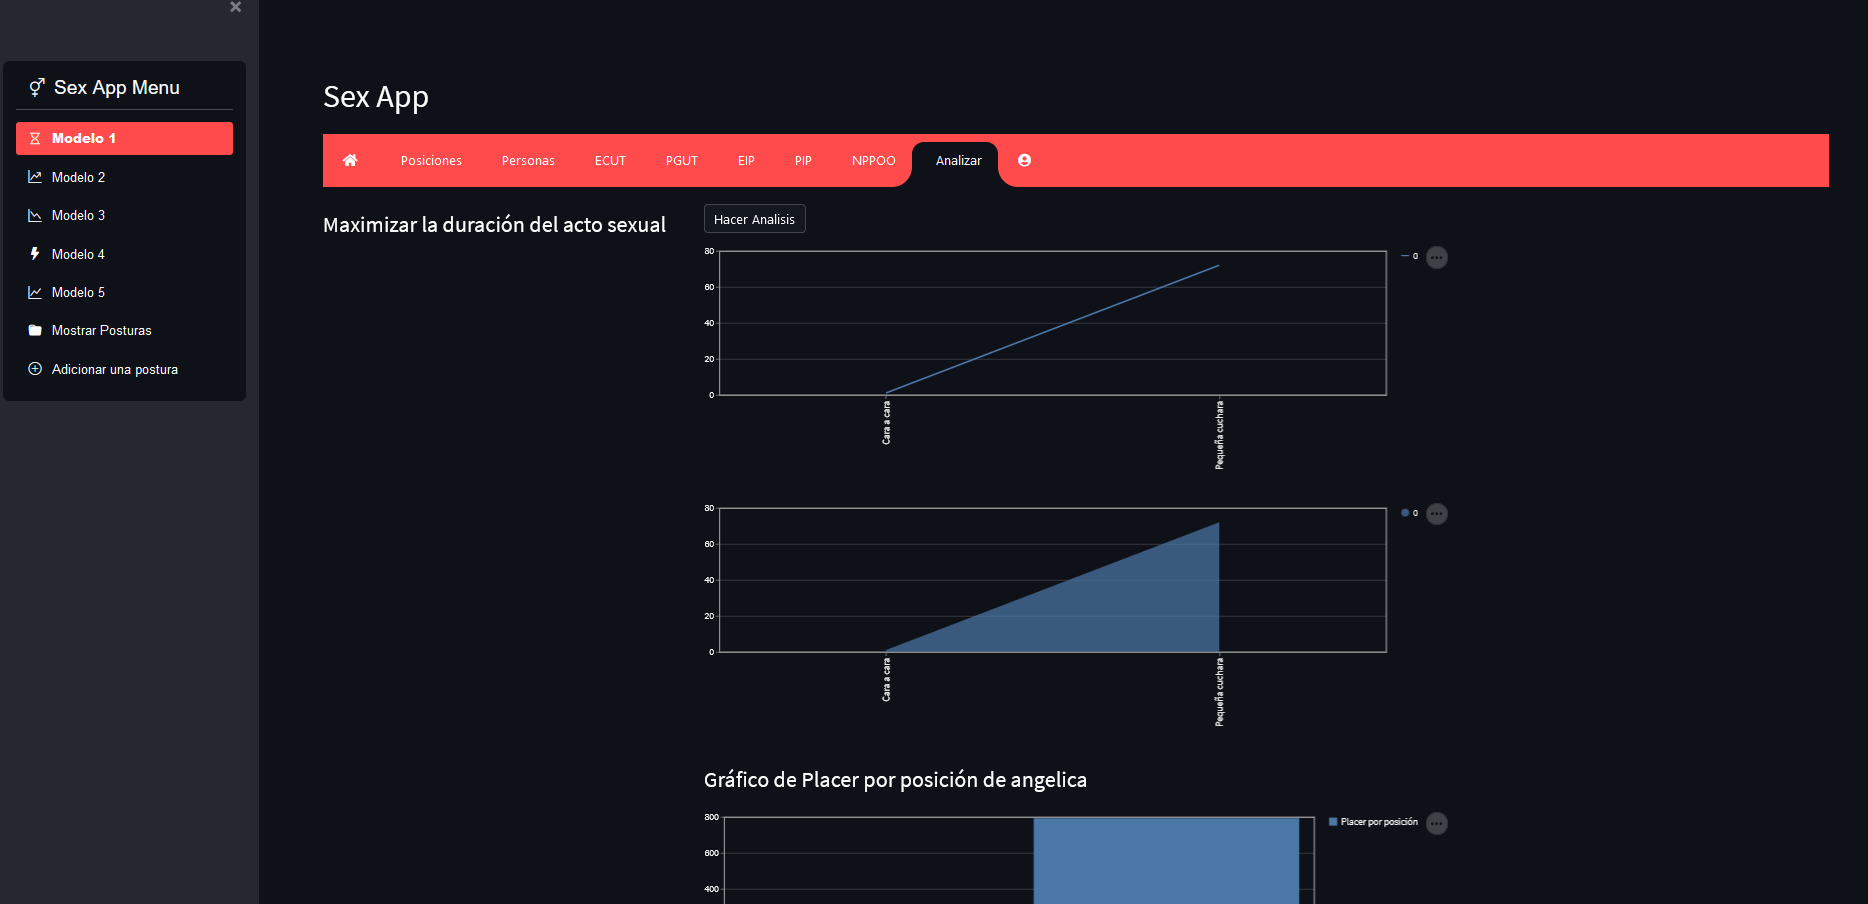
\includegraphics[width=0.7\linewidth]{Imagenes/aplicacion/modelo1analizar}
	\label{fig:modelo1analizar}
\end{figure}

En caso que no haya solución mandará un mensaje de que tipo de problema hubo.
\newline
\newline
Para en caso de los otros modelos la forma de proceder será igual

\newpage

\section{Guía de modificación externa del código}
Como decíamos nuestra aplicación se basa en una página web en la que nosotros damos un encabezado a la pagina de la siguiente forma:
\begin{figure}
	\centering
	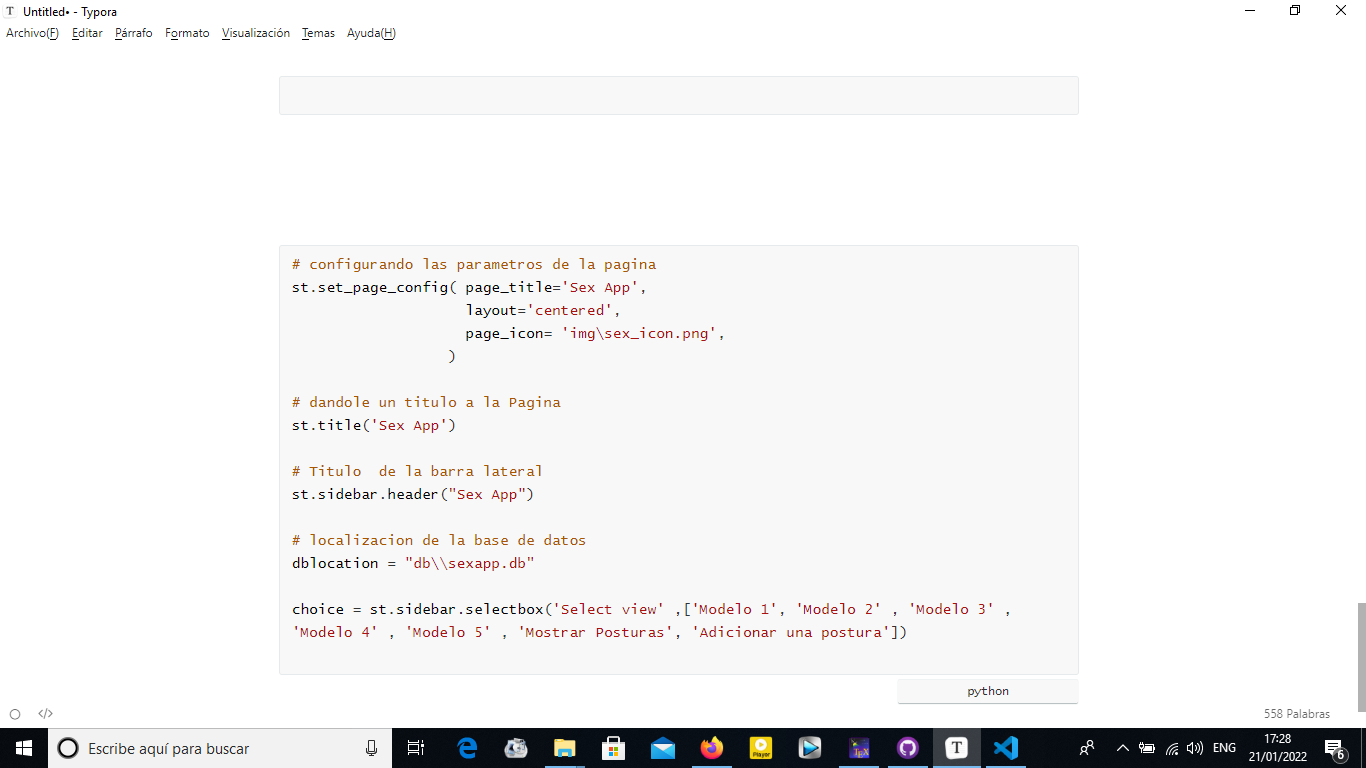
\includegraphics[width=0.7\linewidth]{Imagenes/Codigo-Aplicacion/1}
	\label{fig:1}
\end{figure}
Donde usamos el setpage para poder construir nuestra página web ue tomaría como título, usando el método st.title, el nombre de ´Sex app´.
\newline
\newline
Luego construimos la barra que aparece en la ubicación izquierda de cuando abrimos la página web con st.sidebar.header para poner el nombre de la pagina web y guardar en una variable llamada choice el dato que hayamos escogido en un st.sidebar.selectorbox que es la barra donde seleccionamos un grupo de opciones como lo es Modelo1, Modelo2 y asi sucesivamente.
\newline
\newline
Una vez obtenido el valor escogido pasamos a preguntar que valor tiene escogido el choice de la siguiente manera:

\begin{figure}
	\centering
	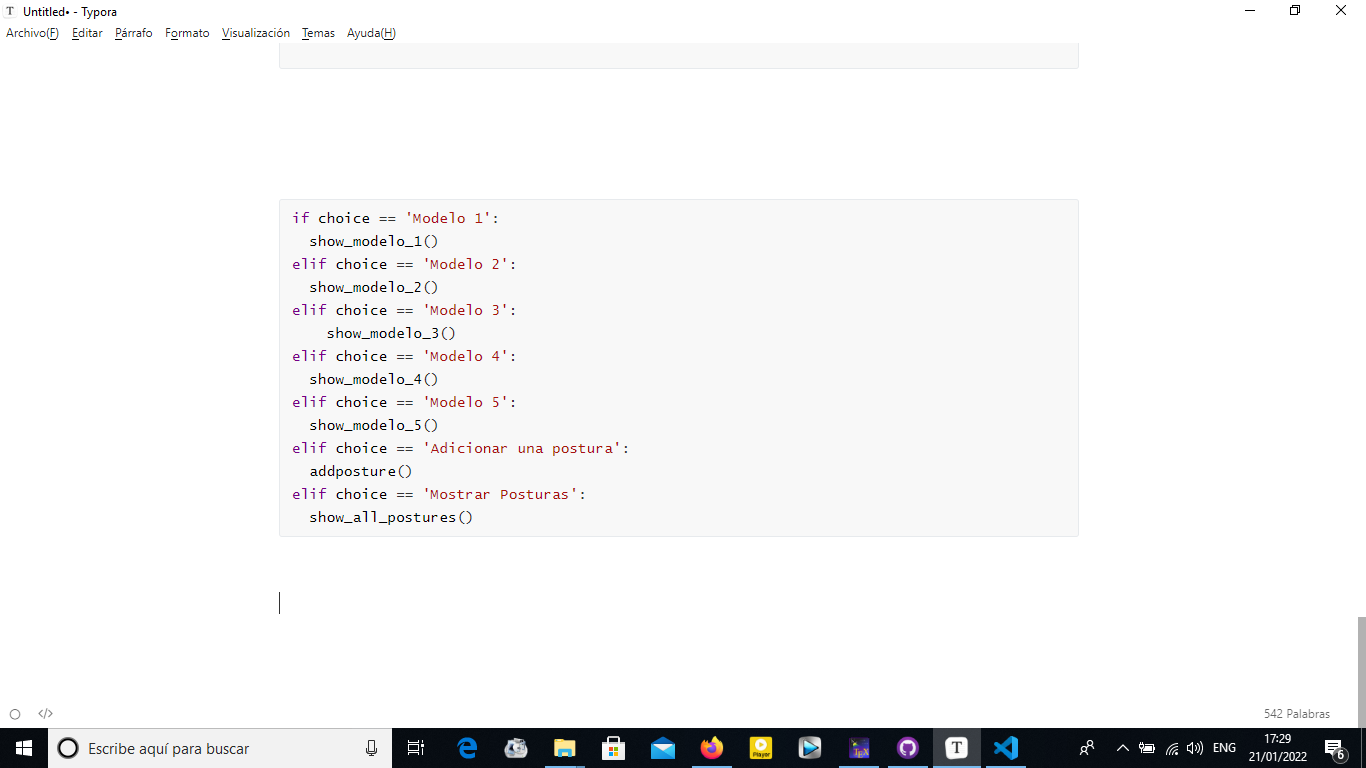
\includegraphics[width=0.7\linewidth]{Imagenes/Codigo-Aplicacion/2}
	\label{fig:2}
\end{figure}

Atendiendo a estas preguntas realizaremos uno de los métodos definidos para realizar la correspondiente elección, en el caso de haber elegido un modelo procederemos a la revisión de un menú que nos sale en la parte superior que nos permitirá cambiar ciertos datos además de darnos el nombre completo de lo que es esa abreviatura y si vamos a Home nos mandará una descripción de la información de lo que quiere estudiar nuestro modelo
\newline
\newline
Esto lo logramos mediante if en preguntas del valor obtenido en un menu donde si obtenemos 'Home' escribiremos el título de nuestro nuevo encabezado con el nombre del modelo que andamos estudiando y una breve descripción de este modelo y si seleccionamos otro nos devolverá un ´subheader´ que mostraremos en próximas imágenes y si es posturas poder seleccionar una postura ya guardada en la base de datos de la aplicación, si es participantes añadimos creamos un formulario para añadir datos de la persona.
\newline
\newline
Ahora explicaremos como usamos los ´subheader´:
\begin{figure}
	\centering
	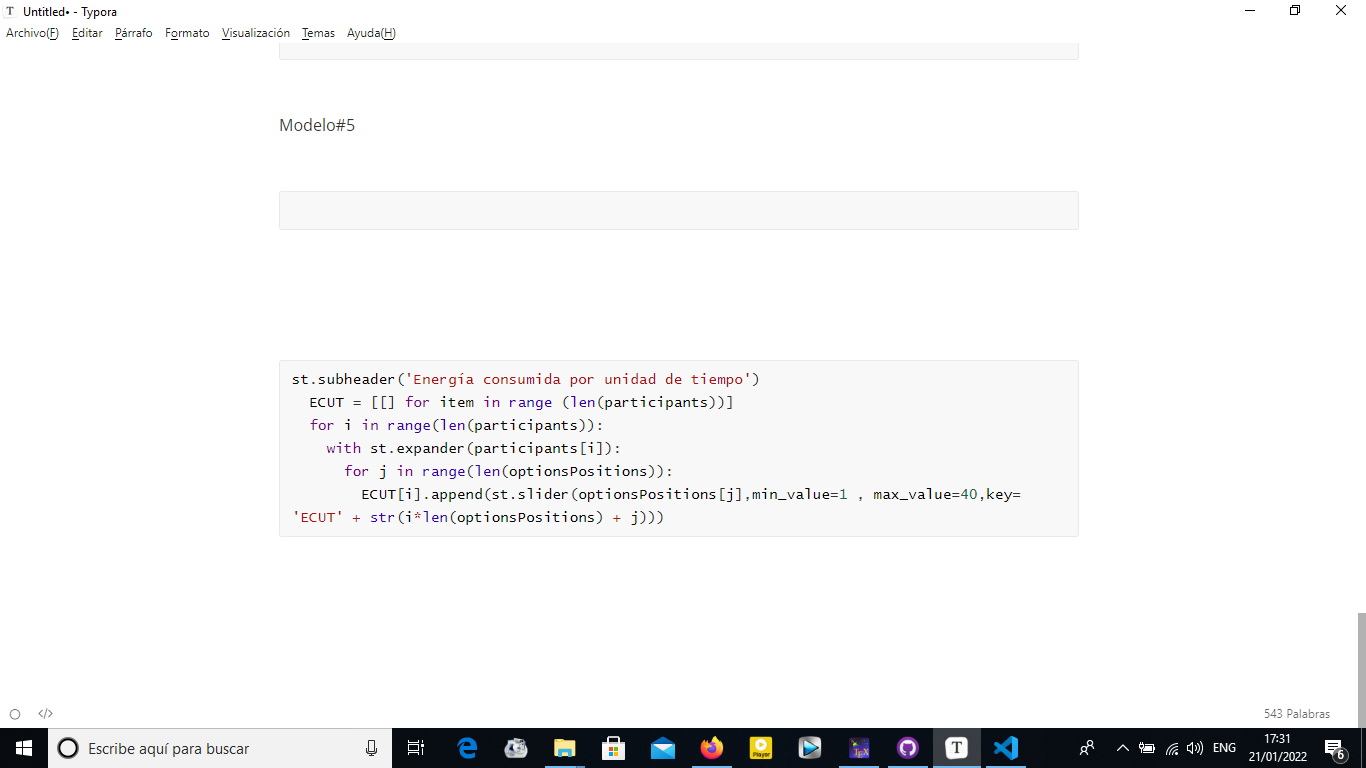
\includegraphics[width=0.7\linewidth]{Imagenes/Codigo-Aplicacion/4}
	\label{fig:4}
\end{figure}
La idea siguiente es crear barra en el que adaptaremos a nuestra conveniencia el valor que creamos a conveniencia del dato que queramos guardar entre un intervalo para luego guardarla en uno de las variables que será la que represente dicho dato en el modelo que estamos trabajando
\newline
\newline
Este código lo repetiremos varias veces a la hora de introducir el EIP, el PGUT y demás datos que nos harán falta para resolver nuestros modelos
\newline
\newline
Luego de añadir todos los datos que queramos aparece en la página un botón llamado analyce, la cual lo usamos en nuestro código luego de la anterior imagen para cuando pulsen el botón empezar a revisar los posibles estados de resultados en nuestro modelo

\begin{figure}
	\centering
	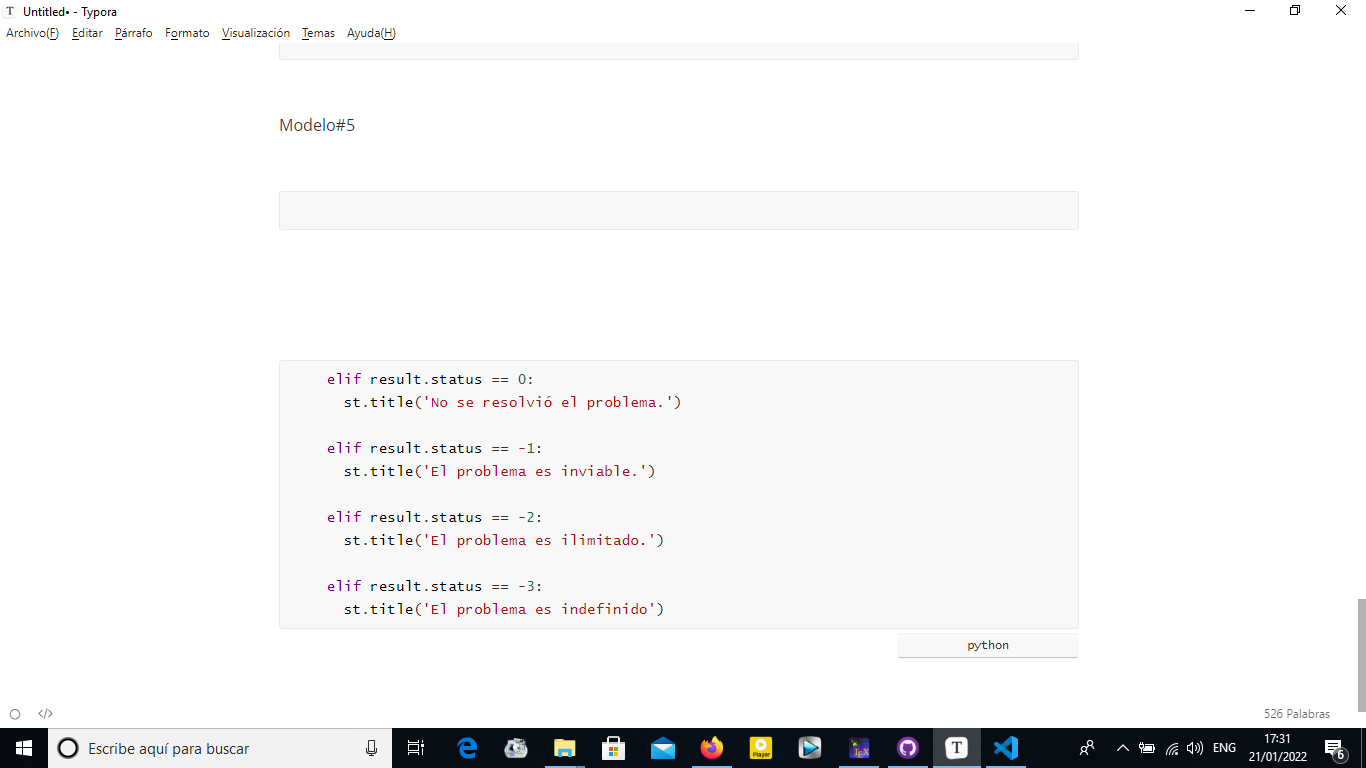
\includegraphics[width=0.7\linewidth]{Imagenes/Codigo-Aplicacion/5}
	\label{fig:5}
\end{figure}
\begin{figure}
	\centering
	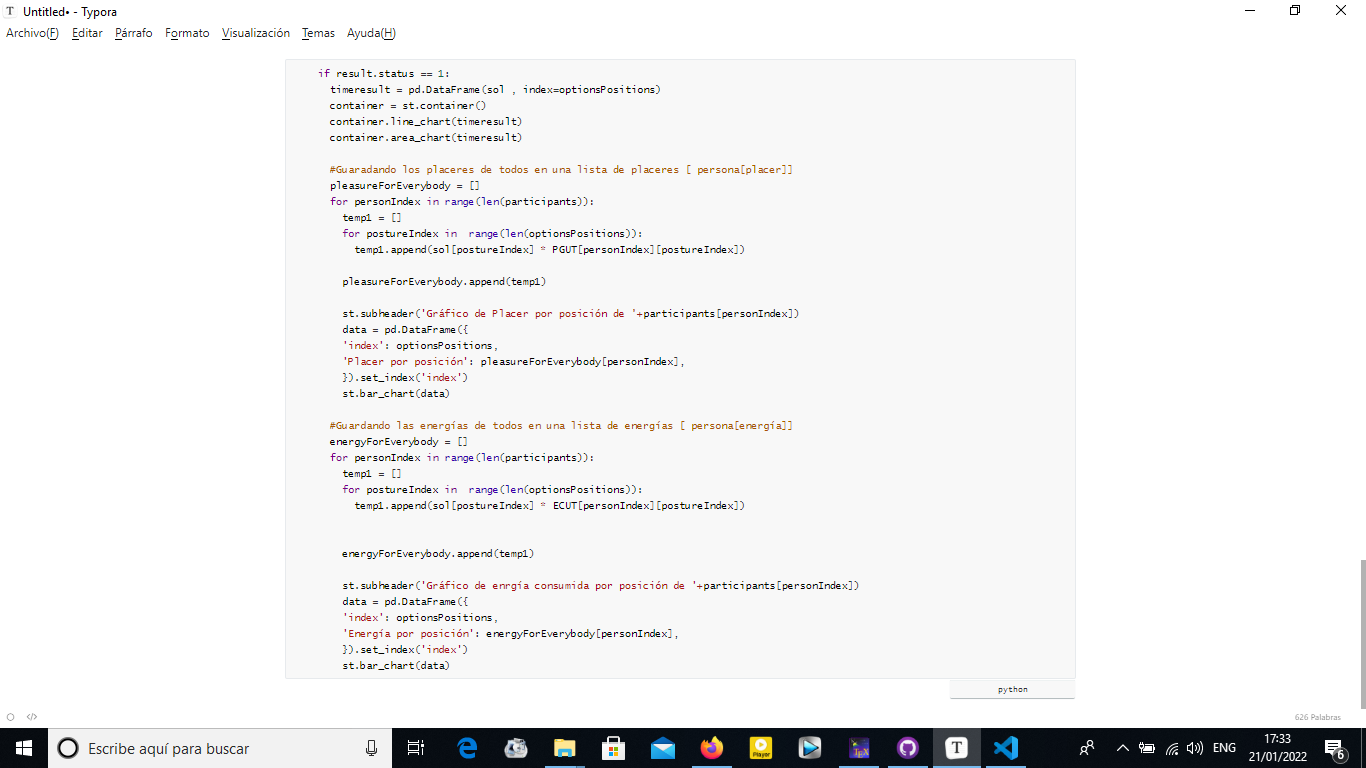
\includegraphics[width=0.7\linewidth]{Imagenes/Codigo-Aplicacion/6}
	\label{fig:6}
\end{figure}

Este último, cuando el estado sea 1, se encargará de imprimir una serie de gráficos vistos en el manual de usuario de la aplicación


\newpage
\section{División organizativa del trabajo}
En este trabajo cada uno trabajo ayudándose mutuamente sin dejar centrarnos en una tarea principal:
\newline
\newline
Daniel de la Cruz: realización de la aplicación por streamlit
\newline
\newline
Dayron Fernández: Análisis y programación de modelos, aportar ideas en la confección de la aplicación, confección de los duales
\newline
\newline
Julio José Horta: Análisis y programación de modelos, aportar ideas en la confección de la aplicación, confección de los duales
\newline
\newline
Javier Villar: Análisis de modelos, ayudar a cada uno de los integrantes en lo que le hiciera falta y confeccionar el Informe


\end{document}
